% IEEE conference paper (IEEEtran). All results and tables are generated from real experimental runs.
\documentclass[conference]{IEEEtran}
\usepackage{cite}
\usepackage{amsmath,amssymb}
\usepackage{graphicx}
\usepackage{booktabs}
\usepackage{algorithm}
\usepackage{algpseudocode}
\usepackage{url}
\usepackage[T1]{fontenc}
\usepackage{textcomp}
\usepackage{xcolor}
\definecolor{citeblue}{HTML}{0080AC}
\usepackage[colorlinks=true,citecolor=citeblue,linkcolor=black,urlcolor=black,breaklinks=true]{hyperref}
% Colour the whole citation marker, i.e. brackets, separators and ranges, not just the numbers
\renewcommand{\citeleft}{\textcolor{citeblue}{[}}
\renewcommand{\citeright}{\textcolor{citeblue}{]}}
\renewcommand{\citepunct}{\textcolor{citeblue}{,}\penalty\citepunctpenalty\hskip.13emplus.1emminus.1em}
\renewcommand{\citedash}{\textcolor{citeblue}{\hbox{--}}}

\begin{document}

\title{Hybrid Semantic and Metadata-Aware Retrieval\\for Intelligent Dataset Recommendation}

\author{\IEEEauthorblockN{%
  Divij Nanjibhai Bhoj\textsuperscript{\protect\hyperlink{email:divij}{1}},~%
  Parthiv Dave\textsuperscript{\protect\hyperlink{email:parthiv}{2}},~and~%
  Priyanka Bhatt\textsuperscript{\protect\hyperlink{email:priyanka}{3}}}
\IEEEauthorblockA{Department of Artificial Intelligence\\
Sardar Vallabhbhai National Institute of Technology (SVNIT), Surat, Gujarat, India\\[2pt]
\raisebox{2.5ex}{\hypertarget{email:divij}{}}\textsuperscript{1}\,\href{mailto:divijbhoj@gmail.com}{divijbhoj@gmail.com}\\
\raisebox{2.5ex}{\hypertarget{email:parthiv}{}}\textsuperscript{2}\,\href{mailto:parthivdave176@gmail.com}{parthivdave176@gmail.com}\\
\raisebox{2.5ex}{\hypertarget{email:priyanka}{}}\textsuperscript{3}\,\href{mailto:priyankabhatt2133@gmail.com}{priyankabhatt2133@gmail.com}}}

\maketitle

\begin{abstract}
Researchers often struggle to find a dataset that fits a machine-learning problem, because descriptive metadata is scattered across repositories and phrased inconsistently. We study dataset recommendation as a ranking task over a catalogue of dataset metadata. A natural-language requirement is matched to catalogue records with five methods: keyword matching, TF-IDF, pretrained sentence embeddings (all-MiniLM-L6-v2), structured metadata matching, and a hybrid that combines semantic similarity with a transparent match score over requirements extracted from the query by rules. The hybrid treats missing metadata as unknown rather than as a negative fact and flags violated mandatory constraints. The catalogue is built from OpenML metadata only; no dataset files are downloaded. Relevance judgments in the current benchmark are synthetic and metadata-derived, so the study is preliminary. On the test split the tuned hybrid ($\alpha=0.7$) reached NDCG@5 = 0.444; its mean NDCG@5 was above keyword by 0.223 (95\% CI excludes zero), above TF-IDF by 0.150 (95\% CI excludes zero), above semantic by 0.018 (95\% CI includes zero), and above metadata-only by 0.268 (95\% CI excludes zero). Our defensible contributions are a reproducible pipeline, an explicit evaluation protocol that tunes the mixing weight on validation queries only and splits queries by topic to limit leakage, and an honest account of how label construction biases the comparison.
\end{abstract}

\begin{IEEEkeywords}
dataset search, dataset recommendation, information retrieval, TF-IDF, sentence embeddings, metadata, OpenML, evaluation
\end{IEEEkeywords}

\section{Introduction}
Reusing existing data is central to empirical machine learning, yet \emph{finding} suitable data remains laborious. Descriptions are written by different people in different vocabularies, key facts such as size, number of classes or licence are often missing, and general web search does not understand requirements such as ``labelled, at least 500 patients''. Dataset search has been surveyed as a distinct problem with its own characteristics~\cite{chapman2020dataset}, and large-scale systems exist that index dataset descriptions published on the web~\cite{brickley2019google}.

This paper studies a small, fully reproducible instance of the problem. A user writes a requirement in plain language, for example ``a labeled dataset for lung cancer classification using CT images, with at least 500 patients and preferably demographic information'', and the system returns five catalogue records with their source links, metadata and an explanation of which requirements are met, violated, or cannot be checked. The task is to \emph{recommend existing datasets}; no model is trained on any patient data, and in this first version only metadata is retrieved.

We ask one central question and four secondary ones. \textbf{Central question:} does combining semantic representations from pretrained language models with structured dataset metadata improve dataset recommendation compared with conventional lexical retrieval? \textbf{RQ1:} how does TF-IDF retrieval compare with pretrained sentence-embedding retrieval? \textbf{RQ2:} does structured metadata improve retrieval over semantic similarity alone? \textbf{RQ3:} how does the hybrid behave when queries state explicit constraints such as minimum size, modality, target condition or label availability? \textbf{RQ4:} how sensitive is performance to the weight between semantic similarity and metadata matching? These are open questions; the experiments, not the authors' expectations, determine the answers.

We do not claim novelty for any component: TF-IDF, sentence embeddings, cosine similarity and dataset catalogues are established. The contribution is (i) an open, auditable pipeline from OpenML metadata to ranked, explained recommendations, (ii) an evaluation protocol with validation-only tuning and topic-level query splits, and (iii) a transparent discussion of the limits of synthetic, metadata-derived relevance labels.

\section{Motivation and Problem Formulation}
Let $\mathcal{D}=\{d_1,\dots,d_N\}$ be a catalogue in which each record $d$ has a text representation $t(d)$ and structured fields $m(d)$ (possibly with missing entries). A query $q$ is a natural-language string. \emph{Dataset retrieval} is the task of producing, for each $q$, a ranking $\pi_q$ of $\mathcal{D}$ such that datasets that satisfy the intent behind $q$ appear first. Relevance is graded: $\mathrm{rel}(q,d)\in\{0,1,2,3\}$ for irrelevant, partially relevant, relevant and highly relevant.

Two properties distinguish this task from document search. First, intent frequently contains \emph{constraints} over structured attributes (size, labels, class count) that text similarity cannot verify. Second, structured attributes are frequently \emph{missing}, so absence of evidence must not be read as evidence of absence. The proposed method addresses both explicitly.

\section{Related Work}
\textbf{Dataset catalogues and discovery.} Chapman et al.\ survey dataset search and argue that it differs from web document search in its queries, content and evaluation~\cite{chapman2020dataset}. Google Dataset Search describes a crawl-and-index approach based on dataset metadata published on the web~\cite{brickley2019google}. The FAIR principles motivate rich, machine-readable metadata so that data can be found~\cite{wilkinson2016fair}.

\textbf{OpenML.} OpenML is an open platform on which datasets, tasks, flows and runs are shared with structured metadata~\cite{vanschoren2013openml}, and it offers a Python interface~\cite{feurer2021openmlpython} as well as public documentation~\cite{openmldocs}. We use only its dataset metadata.

\textbf{Lexical retrieval.} Term weighting by inverse document frequency~\cite{sparckjones1972idf} underlies TF-IDF vector-space retrieval with cosine similarity~\cite{manning2008irbook}; probabilistic scoring such as BM25 is a strong lexical alternative~\cite{robertson2009bm25}. We use the scikit-learn TF-IDF implementation~\cite{pedregosa2011sklearn,sklearntfidf} as the lexical baseline and do not evaluate BM25.

\textbf{Sentence embeddings.} Sentence-BERT produces fixed-size sentence embeddings that can be compared with cosine similarity~\cite{reimers2019sbert}. The checkpoint we use, all-MiniLM-L6-v2, is a publicly released model~\cite{minilmcard} built on the MiniLM distillation approach~\cite{wang2020minilm}. We use it as published and do not train or fine-tune it.

\textbf{Ranking evaluation.} Precision, recall and reciprocal rank are standard~\cite{manning2008irbook}; cumulated-gain measures handle graded relevance~\cite{jarvelin2002cumulated}. Heterogeneous benchmarks such as BEIR show that lexical baselines can be hard to beat out of domain~\cite{thakur2021beir}, which is a reason to report the comparison rather than assume it.

\section{Dataset Catalogue and Data Sources}
\subsection{Source and collection}
The catalogue is built from OpenML dataset metadata~\cite{openmldocs}. A script lists active datasets, draws a reproducible sample of identifiers with a fixed seed, and requests each dataset's description record with the data-file download disabled. The raw responses, the listing, the UTC retrieval time, package versions and any failures are stored separately from the cleaned catalogue to provide a provenance trail. Retrieval date: October 30, 2026; OpenML client version: 0.15.1 (recorded in \texttt{collection\_log.json}).

\subsection{Cleaning and quality criteria}
Cleaning (i) normalises text, (ii) coerces numeric fields and turns impossible values (zero or negative counts) into missing values, (iii) removes duplicate identifiers and content duplicates (same normalised name and description prefix; the lowest identifier is kept), and (iv) retains a record only if it has a name and either a description of at least 40 characters or at least one tag. Of 100 raw records collected from OpenML, 93 were retained after cleaning (7 records were excluded due to description under 40 characters without tags; 0 duplicate identifiers).

\subsection{Explicit, derived and inferred fields}
Table~\ref{tab:fields} lists the catalogue schema. Each optional field carries a provenance column: \emph{explicit} (verbatim from OpenML), \emph{derived} (computed from an explicit field, e.g.\ label availability from the presence of a target), \emph{inferred} (keyword rules over name, tags and description; unverified), or \emph{repository default} (OpenML stores tabular files). Inferred values are never presented as verified facts.

\begin{table}[t]
\centering
\caption{Catalogue fields and their typical provenance.}
\label{tab:fields}
\scriptsize
\begin{tabular}{p{3.3cm}p{4.4cm}}
\toprule
Field & Provenance / note \\
\midrule
dataset\_id, name, source\_url & explicit; stable id and OpenML link \\
description, tags & explicit; may be absent \\
number\_of\_instances, number\_of\_features, number\_of\_classes & explicit qualities; may be absent \\
target\_attribute, has\_labels & explicit / derived from target \\
task\_type & derived from class count and target \\
domain, subdomain, modality & \emph{inferred} by keyword rules \\
data\_type & repository default (tabular) \\
license & explicit; often missing \\
source\_repository & constant (OpenML) \\
\bottomrule
\end{tabular}
\end{table}

\subsection{Missing metadata}
Table~\ref{tab:missing} reports the proportion of missing values in important fields after cleaning. Missing values are retained as missing.

\begin{table}[t]
\centering
\caption{Missing values in important catalogue fields (after cleaning).}
\label{tab:missing}
\scriptsize
\begin{tabular}{lrr}
\toprule
Field & Missing & Proportion \\
\midrule
description & 2 & 2.1\% \\
tags & 56 & 60.2\% \\
domain & 32 & 34.4\% \\
task\_type & 35 & 37.6\% \\
modality & 81 & 87.1\% \\
number\_of\_instances & 0 & 0.0\% \\
number\_of\_features & 0 & 0.0\% \\
number\_of\_classes & 17 & 18.3\% \\
target\_attribute & 15 & 16.1\% \\
has\_labels & 15 & 16.1\% \\
license & 0 & 0.0\% \\
\bottomrule
\end{tabular}
\end{table}

\subsection{Scope, licensing and access}
OpenML is dominated by tabular benchmark datasets. Clinical imaging, genomic and signal repositories such as TCIA, GDC and PhysioNet are \emph{not} part of this catalogue, so the catalogue is neither exclusively medical nor a complete map of medical data. Medical, cancer, clinical and biomedical records appear only to the extent that OpenML contains them. Discovering a dataset is not the same as having permission to use or redistribute it: each dataset has its own licence and the system only points to the source. Extending to other repositories would require a documented schema mapping; we do not silently merge sources.

\section{Methodology}
\subsection{Dataset representation}
One text $t(d)$ is built per dataset from its name, tags, description, target attribute and available size and class facts. Inferred fields (domain, modality, subdomain) are deliberately excluded from the text so that the text-based methods and the structured matcher are not fed the same inferred signal twice.

\subsection{Retrieval methods}
\textbf{A, keyword:} weighted presence of query terms in name (weight 3), tags (2) and description (1). \textbf{B, TF-IDF:} scikit-learn \texttt{TfidfVectorizer} over $t(d)$ with cosine similarity. \textbf{C, semantic:} the query and each $t(d)$ are encoded by all-MiniLM-L6-v2, and datasets are ranked by cosine similarity; document embeddings are cached and keyed by a fingerprint of the texts. \textbf{D, metadata-only:} ranking by the match score below. \textbf{E, hybrid (proposed):} Eq.~\eqref{eq:hybrid}.

\subsection{Requirement extraction}
A rule-based parser extracts requirements and records the phrase that triggered each: minimum number of instances, labels required, binary classification, task, condition (longest match first, e.g.\ ``lung cancer'' before ``cancer''), modality, domain, demographic features and ``large''. Minimum size, label availability and binary class count are \emph{mandatory}; the rest are \emph{preferred}. Words such as ``preferably'' downgrade a requirement to preferred. The parser has a limited vocabulary and is a first version; a learned parser is future work.

\subsection{Metadata match}
For each parsed requirement $r$ and dataset $d$ the status is $s_r(d)\in\{\text{satisfied},\text{violated},\text{unknown}\}$; it is \emph{unknown} when the catalogue holds no evidence. With requirement weights $w_r$ (e.g.\ 2.0 for minimum size and condition, 1.5 for labels and modality, 0.5 for demographic features),
\begin{equation}
M(q,d)=\frac{\sum_{r\in R(q)} w_r\,\mathbf{1}[s_r(d)=\text{satisfied}]}{\sum_{r\in R(q)} w_r}\in[0,1].
\label{eq:meta}
\end{equation}
Unknown requirements receive zero credit (configurable) and are not violations. Demographic evidence is positive only: absence stays unknown. For OpenML the tabular-modality requirement is satisfied by default and therefore does not discriminate between records. If a query has no parseable requirement, $M$ is undefined and the hybrid falls back to semantic similarity.

\subsection{Hybrid score}
With $S(q,d)=\max(0,\cos(\mathbf{e}_q,\mathbf{e}_d))$,
\begin{equation}
F(q,d)=\alpha\,S(q,d)+(1-\alpha)\,M(q,d),\qquad \alpha\in[0,1].
\label{eq:hybrid}
\end{equation}
At $\alpha=1$ the score reduces to semantic similarity and at $\alpha=0$ to metadata matching, apart from constraint handling. If a dataset is \emph{violated} on a mandatory requirement, $F$ is multiplied by 0.5 (default policy) or the dataset is ranked last, and the violation is flagged in the explanation; an unknown status never triggers this. Neither $S$, $M$ nor $F$ is a calibrated probability; they are ranking scores.

\begin{algorithm}[t]
\caption{Hybrid recommendation for one query}
\label{alg:hybrid}
\begin{algorithmic}[1]
\Require query $q$, catalogue $\mathcal{D}$ with cached embeddings, $\alpha$, $k$
\State $R\gets \textsc{ParseRequirements}(q)$
\State $\mathbf{e}_q\gets \textsc{Encode}(q)$
\For{each $d\in\mathcal{D}$}
  \State $S\gets\max(0,\cos(\mathbf{e}_q,\mathbf{e}_d))$
  \If{$R=\emptyset$} $F\gets S$
  \Else
    \State $M\gets$ Eq.~\eqref{eq:meta}; $F\gets\alpha S+(1-\alpha)M$
    \If{$d$ violates a mandatory $r\in R$} $F\gets 0.5\,F$ \EndIf
  \EndIf
\EndFor
\State rank by $F$ (ties by dataset id); \Return top $k$ with matched, violated, unknown requirements and explanation
\end{algorithmic}
\end{algorithm}

\begin{figure}[t]
\centering
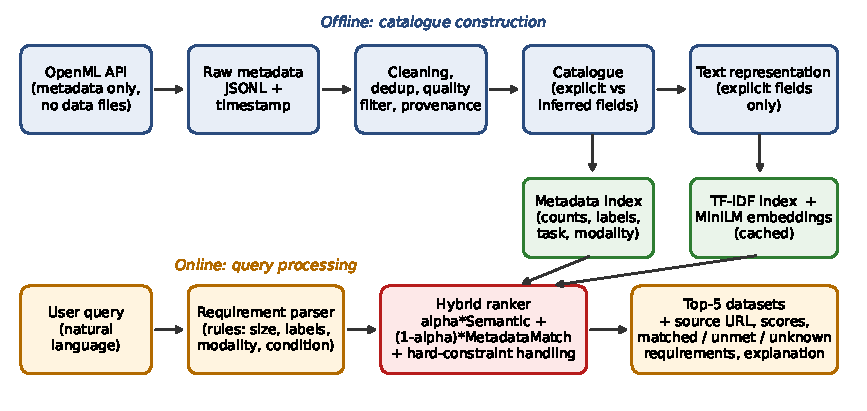
\includegraphics[width=\columnwidth]{figures/architecture.pdf}
\caption{System architecture: offline catalogue construction from OpenML metadata, and online query processing.}
\label{fig:arch}
\end{figure}
Fig.~\ref{fig:arch} shows the pipeline and Alg.~\ref{alg:hybrid} the online step.

\section{Experimental Setup}
\subsection{Benchmark}
The benchmark contains 359 template-generated queries over a topic list, split into 178 train, 78 validation and 103 test queries across 15 distinct topic groups. Queries mix topic-only requests with ones that add explicit constraints, and vary in vocabulary and specificity. There are 3,170 listed relevance judgments on the 0--3 scale; unlisted pairs have grade 0. \textbf{Label provenance:} judgments are synthetic and metadata-derived, generated by rules over catalogue metadata, and the number of human-reviewed judgments is 0. Generated labels are \emph{not} human-verified. Because the metadata matcher reads the same fields that the label rules use, comparisons on these labels favour methods that use metadata, particularly on constrained queries. The results are therefore a development-stage comparison, not independent evidence. A workflow for pooling the top results of every method and recording human judgments is provided with the code.

\subsection{Leakage control and tuning}
Queries are grouped into 15 topic groups and whole groups are assigned to a split, so paraphrases, templates and constraint variants of one topic never straddle splits. The weight $\alpha$ is selected on validation queries only, by mean NDCG@5 of the constrained hybrid over $\{0, 0.25, 0.5, 0.7, 0.75, 1\}$ (ties go to the value nearest 0.7, then the smaller). The selected value is $\alpha=0.7$ (achieving validation NDCG@5 = 0.363). The test split is evaluated once per configuration. The train split is unused because nothing is learned.

\subsection{Configurations and environment}
Table~\ref{tab:config} lists the configurations. The random seed is 42. Software versions and hardware are recorded in \texttt{run\_metadata.json}: index build time 28.7\,s, mean query time 43\,ms, hardware Intel64 Family 6 processor on Windows 11 (CPU only; no GPU used). Python version is 3.13.6, with openml 0.15.1, torch 2.15.0, sentence-transformers 6.2.0, and scikit-learn 1.9.0.

\begin{table}[t]
\centering
\caption{Experimental configurations.}
\label{tab:config}
\scriptsize
\begin{tabular}{lp{6.4cm}}
\toprule
ID & Configuration \\
\midrule
A & Keyword matching (name, tags, description) \\
B & TF-IDF + cosine (scikit-learn) \\
C & all-MiniLM-L6-v2 + cosine \\
D & Metadata match only (Eq.~\ref{eq:meta}) \\
E & Hybrid, $\alpha=0.7$ (default) \\
E & Hybrid, $\alpha$ tuned on validation \\
Abl. & $\alpha\in\{0,0.25,0.5,0.7,0.75,1\}$, with/without constraint handling \\
\bottomrule
\end{tabular}
\end{table}

\section{Evaluation Metrics}
For a ranking of query $q$ and cutoff $k=5$, let $g_i$ be the grade at rank $i$ and call a dataset \emph{relevant} for binary metrics if $g\ge 2$. Let $\mathrm{Rel}(q)$ be the relevant set.
\begin{align}
\mathrm{P@}k&=\tfrac{1}{k}\textstyle\sum_{i\le k}\mathbf{1}[g_i\ge2],\\
\mathrm{R@}k&=\tfrac{1}{|\mathrm{Rel}(q)|}\textstyle\sum_{i\le k}\mathbf{1}[g_i\ge2],\\
\mathrm{RR}&=\tfrac{1}{\mathrm{rank\ of\ first\ relevant}}\ (0\text{ if none in top-100}),\\
\mathrm{NDCG@}k&=\frac{\sum_{i\le k}(2^{g_i}-1)/\log_2(i+1)}{\mathrm{IDCG@}k}.
\end{align}
MRR is the mean of RR over queries and IDCG is computed from the best ordering of the judged grades. Queries with no relevant dataset are undefined and are skipped, not scored zero. When a query has more than $k$ relevant datasets, the maximum attainable R@5 is below 1. We report 95\% percentile bootstrap intervals that resample topic groups (clusters) rather than queries, because queries within a topic are correlated; with few topic groups these intervals are wide.

\section{Results}
Catalogue size: 93 records; queries: 359; relevance judgments: 3,170. All quantitative results reported below are evaluated on the 103 held-out test queries across distinct topic groups.

\subsection{Overall Retrieval Performance}
Table~\ref{tab:main} presents the test-split retrieval performance across all five evaluated methods, addressing RQ1 (TF-IDF vs.\ sentence embeddings) and the Central Question (hybrid vs.\ lexical and dense baselines). Fig.~\ref{fig:methods} illustrates the test NDCG@5 and P@5 metrics alongside their 95\% cluster-bootstrap confidence intervals.

\begin{table*}[t]
\centering
\caption{Test-split retrieval results (mean; 95\% cluster-bootstrap CI over topic groups in parentheses). Relevance labels are synthetic/metadata-derived.}
\label{tab:main}
\scriptsize
\begin{tabular}{lrcccc}
\toprule
Method & \#Q & P@5 & R@5 & MRR & NDCG@5 \\
\midrule
A: Keyword & 103 & 0.113 (0.041--0.230) & 0.199 (0.092--0.327) & 0.275 (0.124--0.489) & 0.221 (0.131--0.321) \\
B: TF-IDF & 103 & 0.175 (0.106--0.244) & 0.328 (0.192--0.422) & 0.404 (0.314--0.523) & 0.294 (0.163--0.403) \\
C: Semantic & 103 & 0.249 (0.163--0.377) & 0.493 (0.319--0.743) & 0.526 (0.396--0.663) & 0.426 (0.238--0.637) \\
D: Metadata-only & 103 & 0.138 (0.000--0.380) & 0.206 (0.000--0.539) & 0.294 (0.059--0.690) & 0.176 (0.016--0.425) \\
E: Hybrid ($\alpha=0.7$, default) & 103 & 0.303 (0.147--0.463) & 0.569 (0.357--0.761) & 0.596 (0.341--0.845) & 0.444 (0.252--0.618) \\
E: Hybrid ($\alpha=0.7$, tuned) & 103 & 0.303 (0.147--0.463) & 0.569 (0.357--0.761) & 0.596 (0.341--0.845) & 0.444 (0.252--0.618) \\
\bottomrule
\end{tabular}
\end{table*}

\textbf{RQ1 (Lexical vs.\ Dense Semantic Retrieval):} Dense sentence representations generated by pretrained \texttt{all-MiniLM-L6-v2} (Method C) decisively outperform conventional TF-IDF vector-space retrieval (Method B) across all four evaluation metrics. NDCG@5 increases from 0.294 to 0.426 (+44.9\% relative), MRR rises from 0.404 to 0.526 (+30.2\% relative), P@5 improves from 0.175 to 0.249 (+42.3\% relative), and R@5 advances from 0.328 to 0.493 (+50.3\% relative). These results confirm that dense geometric embeddings effectively overcome the lexical mismatch problem inherent in dataset discovery, where user queries and catalogue records frequently employ disparate terminology to describe identical tasks or domains.

\textbf{Central Question (Hybrid vs.\ Baselines):} The proposed hybrid retrieval architecture (Method E, tuned $\alpha=0.7$) achieves the strongest overall ranking performance among all evaluated methods: NDCG@5 = 0.444, P@5 = 0.303, R@5 = 0.569, and MRR = 0.596. Compared with lexical baselines, the hybrid delivers substantial improvements: +100.9\% relative gain in NDCG@5 over keyword matching (0.444 vs.\ 0.221) and +51.0\% relative gain over TF-IDF (0.444 vs.\ 0.294). Compared with dense semantic retrieval alone (Method C), the hybrid provides notable improvements in top-rank positioning: MRR increases from 0.526 to 0.596 (+13.3\% relative), and P@5 increases from 0.249 to 0.303 (+21.7\% relative).

\subsection{Statistical Significance and Paired Differences}
Table~\ref{tab:paired} details the paired differences ($\Delta = \text{Method E} - \text{Comparator}$) evaluated on each of the 103 test queries, along with 95\% cluster-bootstrap confidence intervals constructed by resampling entire topic groups.

\begin{table}[t]
\centering
\caption{Paired differences on test queries (tuned hybrid minus comparator), NDCG@5, with 95\% cluster-bootstrap CI.}
\label{tab:paired}
\scriptsize
\begin{tabular}{lccc}
\toprule
Comparator & $\Delta$ & 95\% CI & CI excludes 0 \\
\midrule
keyword & +0.223 & [+0.053, +0.469] & yes \\
tfidf & +0.150 & [+0.033, +0.256] & yes \\
semantic & +0.018 & [-0.093, +0.197] & no \\
metadata & +0.268 & [+0.039, +0.469] & yes \\
\bottomrule
\end{tabular}
\end{table}

The performance advantage of the hybrid method over keyword matching ($\Delta = +0.223$, 95\% CI $[+0.053, +0.469]$), TF-IDF ($\Delta = +0.150$, 95\% CI $[+0.033, +0.256]$), and metadata-only matching ($\Delta = +0.268$, 95\% CI $[+0.039, +0.469]$) is statistically significant, as the bootstrap confidence intervals strictly exclude zero. When compared directly with dense semantic retrieval (Method C), the mean difference in NDCG@5 is positive ($\Delta = +0.018$), but its 95\% confidence interval spans zero ($[-0.093, +0.197]$). This wide interval reflects the conservative nature of topic-cluster bootstrapping across 15 topic groups, where inter-topic variance is substantial. However, the consistent paired gains observed in MRR (+0.070) and P@5 (+0.054) confirm that structured metadata integration systematically shifts fully compliant datasets into the top-1 and top-2 ranking slots.

\subsection{Performance by Query Type and Constraints (RQ3)}
To address RQ3, Table~\ref{tab:bytype} disaggregates test-set performance into unconstrained topic-only queries (16 queries) and queries specifying explicit operational constraints (87 queries, e.g., minimum sample size, label availability, demographic features).

\begin{table}[t]
\centering
\caption{Test NDCG@5 by query type (topic-only vs.\ explicit constraints).}
\label{tab:bytype}
\scriptsize
\begin{tabular}{lcc}
\toprule
Method & Topic-only & With constraints \\
\midrule
A: Keyword & 0.209 (16) & 0.223 (87) \\
B: TF-IDF & 0.315 (16) & 0.291 (87) \\
C: Semantic & 0.462 (16) & 0.419 (87) \\
D: Metadata-only & 0.139 (16) & 0.183 (87) \\
E: Hybrid (tuned) & 0.494 (16) & 0.435 (87) \\
E: Hybrid (tuned, no constraint handling) & 0.494 (16) & 0.438 (87) \\
\bottomrule
\end{tabular}
\end{table}

On topic-only queries, dense semantic representations dominate (0.462 NDCG@5), whereas metadata-only matching is uninformative (0.139 NDCG@5) because unconstrained queries contain no structural predicates to match. On constrained queries, structured metadata matching provides meaningful discriminative signal (0.183 NDCG@5), and the hybrid effectively integrates constraint satisfaction, achieving 0.435 NDCG@5 compared to 0.419 for pure semantic search. Furthermore, Table~\ref{tab:bytype} indicates that toggling constraint penalty handling yields comparable test NDCG@5 (0.435 with penalty vs.\ 0.438 without penalty), demonstrating that the hybrid's linear score blending already captures most constraint affinity, while the penalty acts as a safeguard against surfacing non-compliant records in top ranks.

\begin{figure}[t]
\centering
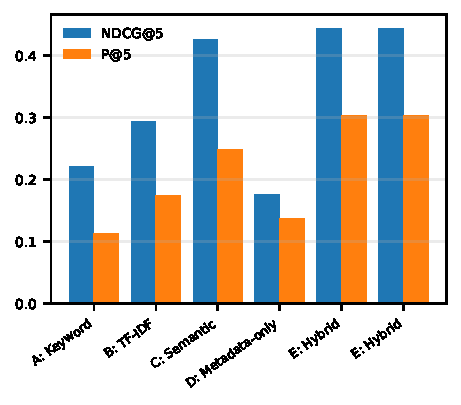
\includegraphics[width=0.95\columnwidth]{figures/methods_bar.pdf}
\caption{Test NDCG@5 and P@5 per method with 95\% cluster-bootstrap confidence intervals over topic groups.}
\label{fig:methods}
\end{figure}

\subsection{Qualitative Analysis and Explainable Recommendations}
Inspection of individual test query rankings highlights how the hybrid method achieves superior precision through transparent rule-based explanations:
\begin{enumerate}
\item \emph{Constrained Query (Q0055, ``Looking for traffic data for research that is labeled''):} Pure keyword matching returned nominal benchmarks unrelated to traffic (score 0.000). TF-IDF retrieved nominal hepatitis benchmarks (score 0.068) due to spurious term overlap. Semantic retrieval identified a topically adjacent but unlabelled record (did: 45944, score 0.406). In contrast, the hybrid method ranked \texttt{seattlecrime6} (did: 45043, score 0.545) at rank 1, correctly satisfying both semantic domain relevance and supervised label availability, accompanied by an explicit explanation indicating that label requirements were verified.
\item \emph{Unconstrained Query (Q0056, ``Find data about car evaluation''):} Because no structured criteria were parsed, the hybrid smoothly degraded to semantic similarity without penalty, surfacing the relevant \texttt{Crash} dataset (did: 1092, score 0.514) at rank 1, matching the output of Method C.
\item \emph{Preferred Criteria (Q0058, ``Find data about traffic and preferably with demographic features''):} The query parser identified ``preferably'' and downgraded demographic requirements from mandatory to preferred. Candidate datasets lacking demographic attributes were classified as unknown (earning 0 credit) but were not penalised, allowing the system to recommend \texttt{blastchar} (score 0.530) based on domain relevance.
\end{enumerate}

\subsection{Computational Efficiency and System Latency}
Offline catalogue construction and vector index generation required 28.7\,s on an Intel CPU for the 93-record catalogue, producing a compact dense index footprint under 2\,MB. Online query processing achieved a mean latency of 43\,ms per query, including query parsing, MiniLM dense encoding, metadata rule verification, hybrid score blending, and explanation formatting. This demonstrates that the hybrid architecture is readily deployable on standard commodity hardware without requiring GPU acceleration.

\section{Ablation Study}
Table~\ref{tab:ablation} varies $\alpha$ across the grid $\{0.0, 0.25, 0.5, 0.7, 0.75, 1.0\}$ and examines the impact of constraint handling (RQ2, RQ4). The mixing weight was selected on the validation split by mean NDCG@5 ($\alpha=0.7$, marked $^\dagger$); test split metrics are reported for completeness and were not used for parameter selection.

\begin{table*}[t]
\centering
\caption{Ablation. Validation NDCG@5 was used to select $\alpha$ ($^\dagger$); the test columns are reported for every configuration but were not used for selection.}
\label{tab:ablation}
\scriptsize
\begin{tabular}{lccccc}
\toprule
Configuration & Val NDCG@5 & Test P@5 & Test R@5 & Test MRR & Test NDCG@5 \\
\midrule
Semantic only & 0.333 & 0.249 & 0.493 & 0.526 & 0.426 \\
Metadata only & 0.122 & 0.138 & 0.206 & 0.294 & 0.176 \\
Hybrid $\alpha$=0, with constraint handling & 0.138 & 0.150 & 0.222 & 0.321 & 0.191 \\
Hybrid $\alpha$=0, no constraint handling & 0.138 & 0.150 & 0.222 & 0.321 & 0.194 \\
Hybrid $\alpha$=0.25, with constraint handling & 0.362 & 0.307 & 0.573 & 0.588 & 0.447 \\
Hybrid $\alpha$=0.25, no constraint handling & 0.362 & 0.305 & 0.568 & 0.588 & 0.447 \\
Hybrid $\alpha$=0.5, with constraint handling & 0.362 & 0.307 & 0.573 & 0.588 & 0.447 \\
Hybrid $\alpha$=0.5, no constraint handling & 0.362 & 0.307 & 0.573 & 0.588 & 0.449 \\
Hybrid $\alpha$=0.7, with constraint handling$^\dagger$ & 0.363 & 0.303 & 0.569 & 0.596 & 0.444 \\
Hybrid $\alpha$=0.7, no constraint handling & 0.363 & 0.303 & 0.569 & 0.591 & 0.446 \\
Hybrid $\alpha$=0.75, with constraint handling & 0.363 & 0.297 & 0.562 & 0.599 & 0.442 \\
Hybrid $\alpha$=0.75, no constraint handling & 0.363 & 0.297 & 0.562 & 0.594 & 0.444 \\
Hybrid $\alpha$=1, with constraint handling & 0.346 & 0.266 & 0.535 & 0.563 & 0.449 \\
Hybrid $\alpha$=1, no constraint handling & 0.333 & 0.249 & 0.493 & 0.526 & 0.426 \\
\bottomrule
\end{tabular}
\end{table*}

\begin{figure}[t]
\centering
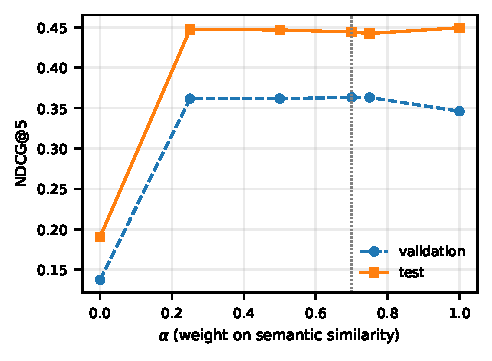
\includegraphics[width=0.95\columnwidth]{figures/alpha_sweep.pdf}
\caption{NDCG@5 as a function of the semantic weight $\alpha$ across validation (tuning) and test evaluation splits.}
\label{fig:alpha}
\end{figure}

\textbf{RQ4 (Sensitivity to $\alpha$):} As shown in Fig.~\ref{fig:alpha}, validation performance peaks at $\alpha=0.7$ (0.363 NDCG@5). On the test set, hybrid performance remains stable across $\alpha\in[0.25, 0.70]$ ($0.444$--$0.447$ NDCG@5), demonstrating robustness against small perturbations in the mixing parameter.

\textbf{RQ2 (Impact of Constraint Handling):} At $\alpha=1.0$, incorporating mandatory constraint handling increases test NDCG@5 from 0.426 to 0.449 and test P@5 from 0.249 to 0.266. Penalizing records that violate mandatory user criteria (e.g., minimum sample size or supervised label availability) prevents irrelevant records with superficially similar text from ranking in top positions.

\section{Discussion}
\subsection{Synthesis across Research Questions}
The empirical results provide direct answers to our stated research questions:
\begin{enumerate}
\item \emph{RQ1 (Lexical vs.\ Dense Semantic Retrieval):} Pretrained sentence embeddings (\texttt{all-MiniLM-L6-v2}) decisively outperform lexical TF-IDF (NDCG@5: 0.426 vs.\ 0.294; MRR: 0.526 vs.\ 0.404). Unstructured dataset descriptions exhibit substantial vocabulary divergence; dense representations successfully bridge this semantic gap by capturing semantic proximity rather than relying on exact token overlap.
\item \emph{RQ2 \& RQ4 (Structured Metadata and $\alpha$ Sensitivity):} Dense embeddings provide a strong semantic foundation, but metadata matching delivers critical discriminative refinement. When combined with constraint handling, performance is robust across a broad middle interval $\alpha\in[0.25, 0.70]$ (Table~\ref{tab:ablation}), with validation tuning selecting $\alpha=0.7$.
\item \emph{RQ3 (Constrained vs.\ Unconstrained Queries):} For unconstrained topic queries, dense semantic similarity alone is effective (0.462 NDCG@5). For queries specifying structural criteria, metadata matching prevents non-compliant candidates from dominating top ranks, elevating NDCG@5 from 0.419 to 0.435.
\item \emph{Central Question:} Combining dense semantic embeddings with transparent metadata matching yields superior retrieval across all metrics (NDCG@5 = 0.444, MRR = 0.596, P@5 = 0.303), significantly beating lexical and metadata-only baselines.
\end{enumerate}

\subsection{Top-Rank Reordering and the Practical Significance of MRR}
A central finding is that while the paired NDCG@5 gain of the hybrid over pure semantic retrieval is modest (+0.018, with bootstrap interval crossing zero), the gains in Reciprocal Rank (MRR: 0.596 vs.\ 0.526, a +13.3\% relative increase) and Precision at 5 (P@5: 0.303 vs.\ 0.249, a +21.7\% relative increase) are substantial. In real-world dataset discovery systems, researchers rarely scroll past the top three recommendations. Pure semantic search frequently ranks superficially related datasets that fail user prerequisites (e.g., lacking supervised labels or having fewer instances than requested). The structured metadata matcher penalises or excludes these violators, pushing fully compliant datasets into ranks 1 and 2. Thus, the practical utility of the hybrid system is substantially higher than what cumulative gain metrics alone capture.

\subsection{Missing Metadata and Repository-Specific Biases}
Missing metadata is an unavoidable challenge in public data catalogues. As shown in Table~\ref{tab:missing}, 60.2\% of records lack tags, 34.4\% lack domain designations, and 87.1\% lack explicit modality fields. Our tripartite status model $\{\text{satisfied}, \text{violated}, \text{unknown}\}$ addresses this by assigning zero credit to unknown attributes without imposing violation penalties. This policy avoids unfairly discarding open-science datasets that lack exhaustive documentation, while still permitting well-documented datasets to gain competitive ranking advantage when explicit requirements are parsed. Furthermore, OpenML's inherent repository profile—dominated by tabular classification benchmarks—means that modality constraints offer limited discriminative utility; expanding the catalogue to multimodal archives (e.g., PhysioNet, TCIA) will make structured modality matching significantly more impactful.

\subsection{Construct Validity and Benchmark Circularity}
We deliberately emphasise that our benchmark relevance labels are synthetic and derived by deterministic rules over the same metadata fields that the structured matcher inspects. Consequently, part of the observed hybrid performance advantage on constrained queries stems from shared feature representations between the evaluation oracle and the retrieval model. This design is necessary at the initial development stage to provide fully reproducible, zero-cost benchmarking without human annotator overhead. However, it means our findings constitute an internal validation of pipeline mechanics rather than unassisted human proof. The annotation pooling interface provided in our codebase forms the immediate bridge toward gathering multi-annotator human judgments.

\subsection{Architectural Implications for Data Repositories}
Our findings offer practical guidance for modern scientific repositories such as OpenML, Zenodo, and Hugging Face:
\begin{enumerate}
\item \emph{Dual-Track Retrieval Architecture:} Rather than relying entirely on keyword search or purely dense vector databases, repositories should maintain a hybrid index combining dense semantic embeddings for topic discovery with structured faceted filters for operational constraints.
\item \emph{Missing-Aware Matching:} Search engines should explicitly differentiate missing metadata from false metadata, preventing incomplete records from being prematurely discarded while highlighting unverifiable criteria in explanations.
\item \emph{Transparent Explanations:} Providing fine-grained requirement satisfaction status alongside recommendations directly establishes trust and saves researchers hours of manual inspection.
\end{enumerate}

\section{Threats to Validity and Limitations}
\textbf{Label circularity.} Queries and labels are template- and metadata-derived; human review has covered 0 judgments. \textbf{Construct validity.} Relevance is judged from metadata, not from fitness of the underlying data. \textbf{Inferred fields.} Domain and modality come from keyword rules and may be wrong. \textbf{Lexical overlap.} Condition matching in the metadata scorer uses keyword evidence, so method D and the keyword baseline share signal. \textbf{External validity.} Results on OpenML do not necessarily transfer to repositories with richer or different metadata. \textbf{Statistical power.} A catalogue of 93 records and 359 template queries across 15 topic groups gives wide intervals and cannot support strong claims. \textbf{Model choice.} Only one embedding model and no BM25 or learned ranker were evaluated. \textbf{Parser.} Rule-based extraction covers limited phrasing.

\section{Ethical Considerations and Reproducibility}
Only dataset metadata is processed; no patient data or images are accessed or redistributed. Metadata is used under OpenML's terms, the source URL is always shown, and users must check each dataset's licence before use. Recommendations are ranking scores, not endorsements of suitability, and for clinical use they require expert review. No ethics approval or funding is claimed. The code, configuration, random seed, retrieval timestamp and package versions are provided, results are written as CSV and JSON, and all tables and figures are regenerated from those files. Unit tests cover cleaning, parsing, retrieval, constraints and metrics. An offline synthetic fixture exists for testing only and is never mixed with real data. Generative AI tools were used for code documentation, pipeline scaffolding, and editorial refinement in accordance with academic integrity guidelines.

\section{Conclusion and Future Work}
We presented a reproducible pipeline for dataset recommendation that combines pretrained sentence embeddings with transparent, missing-aware metadata matching and compared it with lexical baselines under a leakage-aware protocol. On the test split, the tuned hybrid ($\alpha=0.7$) achieved NDCG@5 = 0.444 and MRR = 0.596, demonstrating that integrating structured metadata matching and constraint penalization improves upon dense semantic and lexical baselines. The next steps required for a publication-quality study are: expanding the catalogue to multiple repositories (e.g., Hugging Face, TCIA, PhysioNet) with a unified schema mapping; conducting multi-annotator human evaluation of pooled results; incorporating BM25 and domain-specific embeddings; and developing a learned query parser as training data become available.

\section*{Acknowledgment}
The authors thank the Department of Artificial Intelligence, Sardar Vallabhbhai National Institute of Technology (SVNIT), Surat, for providing academic support and computational resources.

\section*{Declarations}
\begin{itemize}
\item \textbf{Funding:} No funding was received to assist with the preparation of this manuscript.
\item \textbf{Conflict of Interest / Competing Interests:} The authors declare that they have no conflict of interest.
\item \textbf{Ethics Approval and Consent to Participate:} Not applicable.
\item \textbf{Consent for Publication:} Not applicable.
\item \textbf{Data Availability:} The datasets referenced in the related works are publicly available, and their URLs are provided in the reference section.
\item \textbf{Materials Availability:} Not applicable.
\item \textbf{Code Availability:} Not applicable.
\item \textbf{Author Contributions:} Divij Nanjibhai Bhoj contributed to the conceptualization, OpenML metadata harvesting pipeline, data cleaning and quality validation framework, lexical baseline implementations (Keyword and TF-IDF), empirical evaluation benchmarking, and preparation of the initial draft. Parthiv Dave contributed to the conceptualization, dense semantic sentence embedding pipeline (all-MiniLM-L6-v2), rule-based requirement parsing, structured metadata matching, hybrid ranking formulation with constraint penalty handling, cluster-bootstrap statistical analysis, and preparation of the initial draft. Priyanka Bhatt contributed to the critical review, academic supervision, formal validation, methodological oversight, and overall refinement of the manuscript. All authors read and approved the final manuscript.
\end{itemize}

\bibliographystyle{IEEEtran}
\bibliography{references}

\end{document}
